\documentclass[10pt,twocolumn,journal]{IEEEtran}
% XeLaTeX: all fonts are resolved from the local installation.
\usepackage{fontspec}
\defaultfontfeatures{Ligatures=TeX}
\setmainfont[
  BoldFont=TeXGyreTermes-Bold,
  ItalicFont=TeXGyreTermes-Italic,
  BoldItalicFont=TeXGyreTermes-BoldItalic,
  SmallCapsFont=TeXGyreTermes-Regular,
  SmallCapsFeatures={Letters=SmallCaps}
]{TeXGyreTermes-Regular}
\IfFontExistsTF{Arial}{\setsansfont{Arial}}{\setsansfont{Liberation Sans}}
\setmonofont{TeXGyreCursor-Regular}

\usepackage[margin=1in,bottom=1in]{geometry}
% Normal line spacing; content hierarchy provides the space savings.
\setlength{\textfloatsep}{10pt plus 2pt minus 2pt}
\setlength{\dbltextfloatsep}{10pt plus 2pt minus 2pt}
\setlength{\floatsep}{7pt plus 2pt minus 2pt}
\setlength{\abovecaptionskip}{4pt}
\usepackage{xeCJK}
% Build script resolves installed standalone Chinese font files.
% The generated file contains local font paths only; no font binaries are distributed.
\InputIfFileExists{../font_local_zh.tex}{}{%
  \setCJKmainfont[BoldFont=FandolSong-Bold.otf,ItalicFont=FandolKai-Regular.otf,SmallCapsFont=FandolSong-Regular.otf]{FandolSong-Regular.otf}
  \setCJKsansfont[BoldFont=FandolHei-Bold.otf]{FandolHei-Regular.otf}
  \setCJKmonofont{FandolFang-Regular.otf}
}

\usepackage{amsmath,amssymb}
\usepackage{booktabs,array}
\usepackage{graphicx}
\usepackage{xr-hyper}
\usepackage[hidelinks,unicode]{hyperref}
\usepackage{fancyhdr}
\graphicspath{{figures/}}
\setcounter{equation}{13}
\setcounter{table}{4}
\setcounter{figure}{4}
\setlength{\emergencystretch}{2em}
\renewcommand{\topfraction}{0.95}
\renewcommand{\dbltopfraction}{0.95}
\renewcommand{\textfraction}{0.05}
\renewcommand{\floatpagefraction}{0.85}
\renewcommand{\dblfloatpagefraction}{0.85}
\setcounter{topnumber}{3}
\setcounter{dbltopnumber}{3}
\renewcommand{\figurename}{图}
\renewcommand{\tablename}{表}
\DeclareMathOperator{\TV}{TV}
\DeclareMathOperator{\CRPS}{CRPS}
\newcommand{\E}{\mathbb E}
\pagestyle{fancy}
\fancyhf{}
\fancyhead[L]{\scriptsize BELOW ZERO --- SUPPLEMENTARY MATERIAL}
\fancyhead[R]{\scriptsize\thepage}
\renewcommand{\headrulewidth}{0pt}
\hypersetup{pdftitle={Below Zero：补充材料（中文）},pdfauthor={}}
\externaldocument{main}[main.pdf]
\makeatletter\setlength{\@fptop}{0pt}\setlength{\@fpsep}{16pt}\setlength{\@fpbot}{0pt plus 1fil}\makeatother
\newcommand{\BZAuthorBlockEN}{Yaogeng Jiang\\Independent Researcher\\\href{mailto:y.g.jiang@sjtu.edu.cn}{y.g.jiang@sjtu.edu.cn}}
\newcommand{\BZAuthorBlockZH}{姜尧耕\\独立研究者\\\href{mailto:y.g.jiang@sjtu.edu.cn}{y.g.jiang@sjtu.edu.cn}}
\newcommand{\BZPDFAuthors}{Yaogeng Jiang}

\hypersetup{pdfauthor={\BZPDFAuthors}}
\begin{document}
\title{Below Zero：补充材料}
\author{\BZAuthorBlockZH}
\maketitle
\thispagestyle{fancy}

本补充材料提供理论推导说明、网络与训练实现细节、分区域与概率校准分析，以及开发集附加对照实验。公式、表格与图件编号接续正文，全精度评分与源图标识符随附于数据归档中。

\section{单位、条件化与样本的含义}
\subsection{信号与读出}
网络输出 $s\geq0$ 表示以 DN 度量的期望光学信号，对应平均光电子计数 $s/g$。在 $N\sim\operatorname{Poisson}(s/g)$ 下，前向模拟器的整数量化路径为
\begin{equation}
\begin{aligned}
A&=\min\{16383,\lfloor512+gN+\epsilon+b+1/2\rfloor\},\\
V&=A-512.
\end{aligned}
\end{equation}
所有纳入评估的模拟样本均保持在 ADC 物理下界之上。四个 CFA 相位的偏移量在每次实现中独立均匀抽取自 $[-0.25,0.25]$ DN，并作为已知条件同时输入估计器与解码器。

在删失像素处，观测到 $Y_i=0$ 意味着 $V_i\leq0$。在条件独立传感器噪声下，邻近未删失观测为潜在信号 $s_i$ 提供线索，代入估计信号后的条件分布即给出缺失读出的概率分布。

设删失像素处的条件均值与方差分别为 $m=\E[V\mid Y,s]$ 和 $v=\operatorname{Var}(V\mid Y,s)$。对于来自同一条件分布的独立样本 $V'$，有
\begin{align}
\E[(V-m)^2\mid Y,s]&=v,\\
\E[(V-V')^2\mid Y,s]&=2v.
\end{align}
因此，均方误差准则系统性地偏爱抑制读出变异性的条件均值插补 $m$，而非统计分布正确的随机样本 $V'$，这也构成了正文采用恰当概率评分规则的动机。

\subsection{超额评分与已知信号参考}
对于共同离散支撑集上的已知信号条件分布 $p_i^\star$ 与预测分布 $q_i$，期望超额负对数似然等于 KL 散度：
\begin{equation}
\E_{V\sim p_i^\star}[-\log q_i(V)]-H(p_i^\star)=D_{\mathrm{KL}}(p_i^\star\|q_i).
\end{equation}
类似地，展开连续秩概率评分（CRPS）中的平方项可得
\begin{equation}
\begin{split}
&\E_{V\sim p_i^\star}[\CRPS(q_i,V)-\CRPS(p_i^\star,V)]\\
&\qquad=\Delta\sum_k\left(F_{q_i}(k)-F_{p_i^\star}(k)\right)^2.
\end{split}
\end{equation}
这两式将固有的条件读出不确定性与分布估计误差分离，其中已知信号分布 $p_i^\star$ 的自散度与累积差异均为零，但其在含噪读出上的实际 NLL 仍为正值。

对于负值标签 $V<0$，确定性零填充的秩评分为 $|V|$，NLL 为无穷大，正文主表直接报告这些数值。

\section{网络、数据与训练细节}
\subsection{网络架构}
Bayer 相位按 $[R,G_1,G_2,B]$ 打包。16 个输入通道包括四个 $\operatorname{asinh}(Y/4)$ 测量图、四个零候选指示图、四个已知偏移图、一个空间有效性掩码，以及编码 $g$、$\sigma_r$ 和保留零值的三个常量图。掩码区分边界零填充与实测零码，已知偏移同时输入估计器与 PG 解码器。

表~\ref{tab:architecture} 总结了 NAF 风格网络架构。归一化在每个空间位置上跨通道执行（FP32 精度，$\epsilon=10^{-6}$），SimpleGate 将通道维度平分相乘，可学习残差缩放初始化为零。

\begin{table}[t]
\centering\footnotesize
\caption{打包 CFA 坐标下的 N0 架构。}
\label{tab:architecture}
\setlength{\tabcolsep}{3pt}
\begin{tabular}{@{}lccc@{}}
\toprule
阶段 & 宽度 & 模块数 & 空间尺度\\
\midrule
输入 stem & 32 & --- & 1\\
编码器 1 & 32 & 2 & 1\\
编码器 2 & 64 & 2 & 1/2\\
编码器 3 & 128 & 4 & 1/4\\
编码器 4 & 256 & 4 & 1/8\\
瓶颈 & 512 & 4 & 1/16\\
解码器 1--4 & 256/128/64/32 & 各 2 & 1/8 至 1\\
信号输出头 & 4 & --- & 1\\
\bottomrule
\end{tabular}

\vspace{3pt}
\footnotesize 输入含 4 个变换测量图、4 个零指示图、4 个偏移图、1 个有效性掩码和 3 个常量图，输出为 4 个 softplus 信号图。包含 10,913,380 参数的模型不使用池化通道注意力或空间注意力。
\end{table}

嵌套的 128 与 256 像素上下文共享中心 64 像素目标区、偶数 Bayer 对齐与边界有效性掩码，几何翻转与旋转在四相打包前执行。

\subsection{合成分布与划分完整性}
在该校准参数组下，暗帧整数域实测读出噪声方差先减去 $1/12\,\mathrm{DN}^2$，再由模拟器显式执行 1-DN 量化。

1,100 幅渲染 RGB 模板划分为 825 幅训练、137 幅开发与 138 幅测试源图。自然场景抽样（90\%）采用经中位数归一化后在 0.4--64 DN 上对数均匀分布的曝光缩放及 $\exp U[-0.3,0.3]$ 的颜色因子，其中 30\% 叠加 0.1--2 DN 暗部本底，5\% 为零光控制样本，其余 10\% 由程序化图案生成。所有合成设置均独立于实拍曝光。

每幅测试源图生成两个裁剪、增强、曝光与噪声种子均独立的案例。各方法评估完全相同的案例，两种上下文窗口共享同一目标中心，且 bootstrap 重采样将同一源图的四个关联条件始终捆绑为一个重采样单位。

\subsection{优化与精度}
AdamW 采用 $2\times10^{-4}$ 峰值学习率、2,000 次更新预热，并在 80,000 次更新时余弦衰减至 $2\times10^{-6}$，其权重衰减为 0.01，梯度裁剪阈值为 1，滑动平均（EMA）衰减率为 0.999。每次更新累积两个批量为 1 的物理批次，每批次最多向条件交叉熵损失贡献 2,048 个零候选。评测统一采用 seed 7103 在第 80,000 次更新时的 EMA 检查点。

推理时物理解码器由四个预测信号图计算 306 个类别概率。训练采用混合精度，最终网络推理采用关闭 TF32 的完整 FP32 运算，似然与混合积分在需要处采用 FP64。

\subsection{评分汇总与置信区间}\label{sec:scoreaggregation}
像素评分依次在案例内、源图内取平均，最后对源图等权汇总。配对 bootstrap 将每幅源图及其全部案例作为一个重采样单位，整体比较使用 10,000 次重采样。针对 Local Bayes 与 Foi-qPG 的两项预注册主 KL 对比采用 97.5\% 百分位区间（将两项检验的总族错误率控制在 5\%），次要对比采用 95\% 区间。分区域与开发集分析采用未经多重比较校正的逐项 95\% 区间（第~\ref{sec:regionaldefinitions} 节）。所有区间均以固定训练模型为条件，衡量源图抽样变异性。

\section{尾部分辨与概率校准}
查找表（LUT）在 $\log(1+s)$ 与偏移 $b$ 上分别采用 0.002 与 0.01 DN 的步长。在 152 个归档验证查询中，精确解析分布与 LUT 插值分布间的最大 KL 散度为 $2.18\times10^{-7}$ nats，最大质量归一化误差为 $7.77\times10^{-16}$。

\subsection{分辨尾部内的码值}
令 $K=304$，下尾事件为 $T=\{V<-K\}$，LUT 存储的 306 类分布为
\begin{equation}
\bar q=(q(0),q(-1),\ldots,q(-K),q(T)).
\end{equation}
超额 KL 比较归一化粗化分布 $\bar p^\star$ 与 $\bar q$，计入 $T$ 的总概率质量而不区分 $T$ 内部的分布差异。

当抽样命中类别 $T$ 时，第二个独立坐标子流从给定 $T$ 的条件 PG 尾部分布中抽取具体负整数。对于保留的下尾读出码 $k<-K$，其对数概率解析为
\begin{equation}
\log q(k)=\log q(T)+\log p_{\mathrm{PG}}(k)-\log P_{\mathrm{PG}}(T).
\end{equation}
对于贝叶斯混合估计，该解析保留每个信号分量的尾部分布与后验权重，因为直接代入后验均值信号会改变混合尾部形态。

条件矩与秩评分级数求和的截断残差界低于 $10^{-12}$。$-400$ DN 测试验证了混合尾部求值与独立标量分布的一致性，实拍下尾标签同样按其真实整数码解析求值。

\subsection{校准与采样器验证}
表~\ref{tab:coverage} 报告固定 32 源图开发集上的离散等尾区间校准结果，将经验覆盖率与各离散区间实际包含的预测概率质量进行对比。

\begin{table}[t]
\centering\footnotesize
\caption{32 个开发集源图上的离散区间校准。预测值与观测值均为百分数。差值为观测覆盖率减去区间实际包含的预测概率，单位为百分点。}
\label{tab:coverage}
\setlength{\tabcolsep}{3pt}
\begin{tabular}{@{}lrrrrr@{}}
\toprule
方法 & 标称 & 预测 & 观测 & 差值\\
\midrule
N0/PG & 50\% & 52.584 & 52.460 & $-0.123$\\
N0/PG & 80\% & 81.864 & 81.510 & $-0.354$\\
N0/PG & 90\% & 91.819 & 91.685 & $-0.134$\\
N0/PG & 95\% & 97.632 & 97.597 & $-0.035$\\
Local PG & 50\% & 52.177 & 51.962 & $-0.215$\\
Local PG & 80\% & 81.981 & 81.509 & $-0.472$\\
Local PG & 90\% & 91.929 & 91.658 & $-0.270$\\
Local PG & 95\% & 97.639 & 97.538 & $-0.101$\\
已知信号 & 50\% & 52.496 & 52.378 & $-0.118$\\
已知信号 & 80\% & 81.864 & 81.513 & $-0.352$\\
已知信号 & 90\% & 91.854 & 91.725 & $-0.129$\\
已知信号 & 95\% & 97.635 & 97.601 & $-0.034$\\
\bottomrule
\end{tabular}
\end{table}

在固定预测分布与坐标键下，反转处理顺序或按大小 257 分块处理，抽样输出的每个整数均保持不变。所有补全输出均保留正码、以非正整数填充删失候选位置，并在零处再次截断后精确还原输入。

我们在 2,048 个固定预测分布上使用两条随机流及 $S\in\{1,8,32,64\}$ 次抽样验证蒙特卡洛收敛性（参考曲线为 $\sqrt{\operatorname{Var}/S}$）。样本均值 RMSE 从单次抽样的 15.164 DN 降至 64 次抽样的 1.949 DN，吻合 $S^{-1/2}$ 缩放率。在 64 次抽样下，各位置样本方差均值为 227.397 DN$^2$，与解析预测值 226.970 DN$^2$ 一致（两条随机流均已归档）。

\section{输入信息的使用与附加空间分析结果}
\subsection{局部似然与 Bayesian 积分}
对每个同相位邻域 $\mathcal N_i$，记观测码 $t$ 的有效像素计数为 $h_{it}$。局部常值信号似然为
\begin{equation}
\ell_i(s)=h_{i0}\log c(s,b)+\sum_{t>0}h_{it}\log p_Y(t\mid s,b).
\end{equation}
上限饱和以离散上尾概率质量计入似然。Local PG 对网格似然最大值做二次细化，Local Bayes 则结合训练集拟合的零点加 Gamma 信号先验对条件分布进行后验积分，且两者对中心删失事件均只计入一次。信号网格在 32 DN 以下采用约 0.1 DN 间距，32 DN 以上采用 0.5 DN 间距，并除以 $g$ 转换为光电子均值。

N0 利用四相位多尺度上下文，Local/Foi 基线使用同相位观测，而 Joint-CFA Bayes（第~\ref{sec:v3} 节）在 $5\times5$ 窗口内结合四相位观测与有限经验先验。

\subsection{留出区域定义}\label{sec:regionaldefinitions}
留出测试集的分区域剖析采用同相位 $9\times9$ 邻域。令 $u=\log(1+s)$，有效像素上的局部信号变化度定义为 $t=\sqrt{\overline{u^2}-\bar u^2}$。显著梯度位置要求 $u$ 的 Sobel 幅值除以 8 后不低于 0.15（并经 1 像素边界有效性腐蚀），边缘距离定义为打包坐标下的欧氏距离，观测零码比例 $z$ 为有效邻域内 $\mathbf1[Y=0]$ 的均值。

信号分箱边界为 $0,.25,.5,1,2,4,8,16,\infty$ DN，局部变化边界为 $0,.025,.05,.1,.2,.4,.8,\infty$，边缘距离边界为 $0,1,2,4,8,16,\infty$，零码比例边界为 $0,.1,.25,.5,.75,.9,1$。256 像素上下文共含 1,627,306 个唯一候选像素。各源图在各分箱内先合并两案例的评分总和并除以总候选数，再对包含该分箱样本的源图等权平均，逐项 95\% 区间采用 2,000 次成对源图重采样（种子 1280027）。各分箱包含的有效源图数不同（例如 $z\geq0.75$ 分箱仅含来自 1 幅源图的 2 个候选），完整计数与评分见 \path{V9_heldout_spatial_bins_256.csv}。

在最暗分箱 $s<0.25$ DN（含 94 幅源图的 311,545 个候选位置）中，N0 减 Foi-qPG 的平均超额 KL 为 $5.35\times10^{-5}$ nats（区间 $[2.68,9.88]\times10^{-5}$），N0 减 Local Bayes 为 $-8.72\times10^{-5}$ nats（区间 $[-25.0,0.693]\times10^{-5}$），表明均匀近黑区域与结构化区域的表现存在本质差异。

\subsection{开发集绝对误差与匹配对比}
图~\ref{fig:absolutegradient} 报告固定 32 源图开发集在低、中、高梯度组上的源图平均绝对超额 KL，N0 对 Local PG 分别为 $0.000191$ 对 $0.000791$、$0.000249$ 对 $0.001007$ 以及 $0.000442$ 对 $0.002109$ nats。从低梯度到高梯度，成对 KL 差（N0 减 Local PG）的变化量均值为 $-0.001066$ nats（中位数 $-0.000102$，32 幅源图中 23 幅为负，两个最大降幅占净降幅总和的 65.7\%，10,000 次重采样 95\% 区间为 $[-0.002177,-0.000271]$），对应的含噪 NLL 差值变化量为 $-0.000807$ nats（区间 $[-0.003231,0.001221]$，32 幅中 12 幅为负）。

粗信号匹配仅保留同一源图、CFA 相位与信号分箱内同时含至少 5 个低梯度和 5 个高梯度候选像素的单元，在源图内以较小候选数为权重汇总后再对源图等权平均。在 27 幅源图的 142 个匹配单元上，高减低成对 KL 差值变化量均值为 $-0.000268$ nats（中位数 $-0.0000358$，27 幅中 18 幅为负，20,000 次重采样区间 $[-0.000581,-0.0000280]$），NLL 变化量为 $0.000122$ nats（区间 $[-0.002049,0.002086]$）。表~\ref{tab:adverse} 列出了基线更优或区间跨零的区域 NLL 对比。

\begin{figure}[t]
\centering
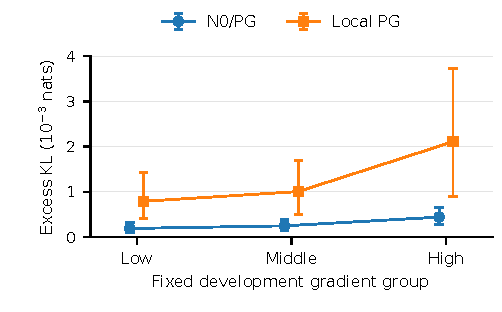
\includegraphics[width=\columnwidth]{s10_absolute_gradient.pdf}
\caption{固定 32 源图开发集上的绝对条件分布误差。各点和 95\% 源图 bootstrap 区间在每个梯度组内采用源图等权。两种误差均随梯度上升，Local PG 增幅更大。该图像集和分组方式与正文图 4 的留出边际比较所用设置不同。}
\label{fig:absolutegradient}
\end{figure}

\begin{table*}[t]
\centering
\caption{基线更优或区间跨零的部分区域 NLL 对比。N0 减基线的差值及逐项 95\% 源图 bootstrap 区间均以 $10^{-3}$ nats 为单位，前两行来自事后留出案例分组，案例零比例 $z_{\mathrm{case}}\geq0.5$，其余行为开发集候选。$d$ 为 $\log(1+s)$ 的 Sobel 幅度除以八，$a$ 为打包坐标下四连通零分量的像素数。}
\label{tab:adverse}
\begin{tabular}{@{}llrrrr@{}}
\toprule
特征 / 分箱 & 比较方法 & 源图数 & 差值 & \multicolumn{2}{c}{95\% 区间}\\
\midrule
案例零比例 $\geq0.5$ & Local Bayes & 30 & $+0.0020$ & $-0.0132$ & $+0.0172$\\
案例零比例 $\geq0.5$ & Foi-qPG & 30 & $+0.0080$ & $-0.0039$ & $+0.0200$\\
信号 $0\leq s<2$ DN & N0 置换 & 28 & $+1.3432$ & $-2.3007$ & $+6.1834$\\
信号 $s\geq16$ DN & Local PG & 20 & $-1.9514$ & $-4.0343$ & $+0.2155$\\
梯度 $0\leq d<0.025$ & Local PG & 32 & $+0.0043$ & $-1.4801$ & $+1.6993$\\
梯度 $0.025\leq d<0.1$ & Local PG & 32 & $+0.1099$ & $-0.9157$ & $+1.2081$\\
梯度 $d\geq0.1$ & Local PG & 32 & $-0.8031$ & $-2.0314$ & $+0.3147$\\
零分量大小 $a\geq33$ & Local PG & 30 & $-0.5950$ & $-2.0038$ & $+0.5810$\\
零分量大小 $a\geq33$ & N0 置换 & 30 & $-0.5265$ & $-3.8384$ & $+3.0659$\\
\bottomrule
\end{tabular}
\end{table*}

\subsection{为什么汇总曲线可能重叠}
由全变差（TV）距离的三角不等式，对各位置预测分布先做空间等权平均会抵消方向相反的逐像素差异：
\begin{equation}
\TV\!\left(\frac1n\sum_iq_i,\frac1n\sum_ir_i\right)
\leq\frac1n\sum_i\TV(q_i,r_i).
\end{equation}
开发集上 N0 与 Local PG 的平均逐点 TV 为 0.01235，而实拍数据空间汇总 PMF 的 TV（依样本集与权重不同）降至 0.000282 和 0.001561。归档逐点直方图保留了完整位置差异，逐位置成对评分则直接评估空间汇总前的预测精度。

\section{真实曝光与下游评价方案}
\subsection{整数对齐与隐藏参考}
\begin{table}[t]
\centering\footnotesize
\setlength{\tabcolsep}{2.2pt}
\caption{排除深尾或重复坐标前后的真实数据评分。表中为共同 R/$G_1$/$G_2$ 候选位置上 N0 减 Local PG 的差值，负值表示 N0 更低。首行为完整样本结果，其余行为依据保留读数划分的子集。}
\label{tab:real_robust}
\begin{tabular}{@{}llrrr@{}}
\toprule
帧 & 纳入的位置 & $N$ & $10^3\Delta$NLL & $\Delta$CRPS (DN)\\
\midrule
4748 & 全部 & 12,652 & $-1.342$ & $-0.01102$\\
 & $V>-128$ & 12,609 & $-1.375$ & $-0.01145$\\
 & 排除重复坐标 & 12,650 & $-1.336$ & $-0.01098$\\
\addlinespace[2pt]
4749 & 全部 & 19,200 & $-0.964$ & $-0.00920$\\
 & $V>-128$ & 19,121 & $-0.998$ & $-0.00927$\\
 & 排除重复坐标 & 19,198 & $-0.945$ & $-0.00907$\\
\bottomrule
\end{tabular}
\end{table}

实拍参考读出采用固定整数变换 $V=R_{\mathrm{native}}-512+n_c$（R/$G_1$/$G_2$/B 的 $n_c=(2,3,3,3)$ DN），原始相机文件保持不变，整数平移完整保留原生量化网格。十幅独立暗帧校准后仍余小数残差 $(-0.437,-0.310,-0.189,+0.078)$ DN。由于推理时输入零偏移，该残差构成实拍模型失配的一部分。

表~\ref{tab:tail_original} 汇总了全部 31,852 个共享实拍 R/$G_1$/$G_2$ 候选位置的零原子与嵌套负尾事件（含固定的 $-125$ DN 诊断阈值，有别于正文及表~\ref{tab:real_robust} 的 $-128$ DN 阈值），第~\ref{sec:realcode} 节将极端负标签追溯至原始码值。

\begin{table}[t]
\centering
\caption{全部 31,852 个共享真实 R/$G_1$/$G_2$ 候选项中的零原子与尾部事件。期望计数为 N0 概率之和，观测计数使用保留的有符号标签。}
\label{tab:tail_original}
\begin{tabular}{@{}lrr@{}}
\toprule
事件 & 期望计数 & 观测计数\\
\midrule
$V=0$ & 1107.76 & 1190\\
$V\leq-1$ & 30744.24 & 30662\\
$V\leq-50$ & 1345.75 & 1065\\
$V\leq-125$ & 0.01690 & 132\\
$V\leq-305$ & $8.63\times10^{-30}$ & 13\\
\bottomrule
\end{tabular}
\end{table}

\subsection{固定的去马赛克路径}
固定的 LibRaw 0.22.1 管线依次调用 \path{open_bayer(black=0)}、\path{unpack}、\path{raw2image_ex(0)}、\path{pre_interpolate} 和 \path{ahd_interpolate}，随后执行 FP32 基座扣除，从而绕过默认的黑电平扣除、缩放、白平衡、色彩/gamma 转换和去噪（版本与补丁哈希均已归档）。负值图案测试证实黑电平以下信息能到达插值阶段，固定源码实现精确复现了全部六个全幅线性 RGB 数组。鉴于 AHD 的非线性决策依赖于基座值（已在 $P=512$ 与 $P=1024$ 下验证），所有对比统一采用 $H(V+512)-512$。

\subsection{A/B/C/D 统计}
每个实拍 ROI 为 $512\times512$ Bayer 像素，去除 16 像素边界后保留 $480\times480$ 个 RGB 像素用于评估。路线 A 和 B 为固定的有符号与截零参考，路线 C 和 D 各自对 32 次独立条件抽样逐一执行去马赛克，先在单次抽样内计算空间统计量再跨抽样取平均。路线 D 在实拍数据上使用预注册的 $3\times3$ Local PG 窗口（合成测试使用 $5\times5$）。

\begin{table*}[t]
\centering
\caption{两次曝光中预先选定的最暗真实 ROI 的线性相机 RGB 统计，位于白平衡或显示钳位之前。A/B 为固定参考，C/D 对 32 个分别去马赛克样本的空间统计取平均。单位为 DN。数据包含全部 12 个 ROI。}
\label{tab:ahd}
\begin{tabular}{@{}llrrrrr@{}}
\toprule
曝光 & AHD 输入 & $\mu_R$ & $\mu_G$ & $\mu_B$ & sd$(R-G)$ & sd$(B-G)$\\
\midrule
P2654748 & A：有符号参考 & 8.041 & 9.003 & 3.200 & 25.986 & 22.037\\
& B：钳位 & 15.368 & 16.322 & 11.707 & 18.635 & 15.127\\
& C：N0 样本 & 7.924 & 8.621 & 1.655 & 25.157 & 22.495\\
& D：Local PG 样本 & 7.933 & 8.602 & 1.642 & 25.256 & 22.587\\
P2654749 & A：有符号参考 & 0.423 & 0.797 & $-0.225$ & 23.584 & 20.529\\
& B：钳位 & 10.089 & 10.287 & 9.146 & 15.243 & 12.712\\
& C：N0 样本 & 0.231 & 0.246 & $-1.871$ & 22.813 & 20.860\\
& D：Local PG 样本 & 0.352 & 0.352 & $-1.812$ & 22.799 & 20.861\\
\bottomrule
\end{tabular}
\end{table*}

表~\ref{tab:ahd} 给出预先选定的两个最暗 ROI（全部 12 个 ROI 均已归档）。跨抽样区间反映补全抽样变异性，单次抽样内的空间标准差则同时反映场景纹理与去马赛克相关性。

\subsection{处理顺序示意}
\href{visual_zh.pdf}{补充图像 A} 展示帧 P2654749 在 $(0,1500)$ 处的 $1000\times1000$ Bayer 区域经全幅 AHD 与 $4\times4$ 面积缩采样至 $250\times250$ RGB 像素后的视觉对比，其中各路线共享曝光与显示变换，仅在 RAW/RGB 截零顺序上不同。

\subsection{基于干净参考的暗部颜色误差评价}\label{sec:cleanendpoint}
本开发集实验方案在前期开发集分析完成之后、计算任何颜色评分之前锁定，明确规定了固定渲染管线与误差指标，且未预设主观感知效果阈值。我们仅依据几何完整性从 32 源图开发集中选取八个自然场景裁剪块（选取过程完全不参考终点颜色评分），另取四个程序化合成模板单独评估。每个场景生成 16 次独立的 PG 传感器噪声实现，每个估计器在每次传感器实现下独立抽取两个条件补全样本。固定渲染管线依次采用基座值 512 的整数 AHD 去马赛克、四倍有符号域面积平均、固定白平衡与相机到显示色彩矩阵，以及由各场景干净参考唯一确定的单一曝光系数。剔除评分边界后，取干净参考亮度最低的八个空间块组成暗部评估区，在曝光缩放后的线性显示 RGB 空间中计算块均值色度向量 $(R-G,B-G)$ 相对于 clean-$Q$-AHD 参考（其中 $Q(s)=\lfloor s+0.5\rfloor$）的平方误差，而确定性条件均值分支同样先按量化算子 $Q$ 量化为整数后再送入 AHD。所有评分均先在单次渲染样本上计算，随后在传感器实现内取平均，最后对八幅自然源图等权汇总。

实验结果显示，N0 条件抽样的暗部颜色误差比 Local PG 条件抽样低 $0.003139$（95\% 源图配对 bootstrap 区间为 $[-0.006136,-0.000843]$），且在全部八幅自然源图上改善方向一致，其中改善幅度最大的两幅源图贡献了总降幅的 67.9\%。若改用量化条件均值补全，N0 的暗部颜色误差较条件抽样再降低 16.5\%。相比之下，在以量化干净信号 $Q(s)$ 为参考的逐像素干净 RAW 均方误差（MSE）上，N0 条件抽样反而比 Local PG 高出 $2.062$ DN$^2$（95\% 源图区间为 $[0.713,3.834]$，八幅源图中仅有一幅有利于 N0）。有符号参考分支直接使用每幅源图 16 次传感器实现各自的未截断含噪读出，而 clean-$Q$-AHD 则是独立的无噪颜色参考，且 N0 条件抽样与未截断有符号分支之间的成对颜色误差差值区间跨零。全部 12 幅测试源图的完整结果、次要指标与逐次抽样记录均已随数据归档，八幅自然源图的汇总评分亦收录于 \texttt{evidence/clean\_color/}\allowbreak\texttt{PER\_SOURCE.csv}。

\section{数值与复现记录}
全画幅分块推理在打包四通道 CFA 坐标系中采用 256 像素核心块与 192 像素重叠扩展边（halo），核心块与扩展边尺寸均为 16 的整数倍，以确保四级编码器--解码器下采样相位完全对齐。输入观测与像素有效性掩码在进入网络前补零至 16 的整数倍，各分块在图像外边界处截断，最终仅拼接保留各分块的核心区预测结果。发布代码在 \path{inference/tiling.py} 中完整实现了上述分块流程。条件抽样按第 III 节所述协议使用全画幅绝对像素坐标作为随机数种子输入，随附证据档案完整保留了数组级复现校验、码值范围记录、解码器标识信息以及隔离环境推理示例的依赖项与验证容差。

\section{附加开发集控制}\label{sec:v3}
以下事后开发集对照实验使用开发集数据，用于补充支撑预注册留出测试集上的结论。

\subsection{Joint-CFA 局部开发集比较方法}
为检验跨通道相关性是否足以解释局部模型的劣势，Joint-CFA local Bayes 从 128 个训练场景各抽取两个四相位模板，构成含 256 个等权四相信号模板的经验先验。该估计器在打包 $5\times5$ 局部窗口内联合计算全部有效四相观测的似然（每个中心或邻域删失像素仅作为删失事件计入一次），并对相应的条件整数 PG 分布进行后验加权混合。我们将 N0 与两种局部估计器在 32 幅开发源图共享的 32,462 个候选位置上进行同口径对比评估。

\begin{table}[t]
\centering\scriptsize
\setlength{\tabcolsep}{2pt}
\caption{在 32 个固定源图上的事后开发集比较。CFA 均值先在源图内计算，再对源图等权。}
\label{tab:joint}
\begin{tabular}{@{}lrrr@{}}
\toprule
方法 & 超额 KL (nats) & NLL (nats) & CRPS (DN)\\
\midrule
N0/PG & 0.000376673 & 3.911227506 & 8.103882756\\
Joint-CFA local Bayes & 0.001790969 & 3.912282251 & 8.112198163\\
同 CFA Local PG & 0.001952344 & 3.912362493 & 8.112870272\\
\bottomrule
\end{tabular}
\end{table}

如表~\ref{tab:joint} 所示，N0 减 Joint-CFA local Bayes 在超额 KL、NLL 与 CRPS 上的成对差值（及 95\% 源图 bootstrap 区间）分别为 $-0.00141430$ nats（$[-0.00296235,-0.00031761]$）、$-0.00105475$ nats（$[-0.00215630,-0.00029750]$）与 $-0.00831541$ DN（$[-0.01755261,-0.00217521]$），而 Joint-CFA local Bayes 减同相位 Local PG 的 NLL 与 CRPS 成对差值置信区间均跨越零点。

\begin{figure*}[t]
\centering
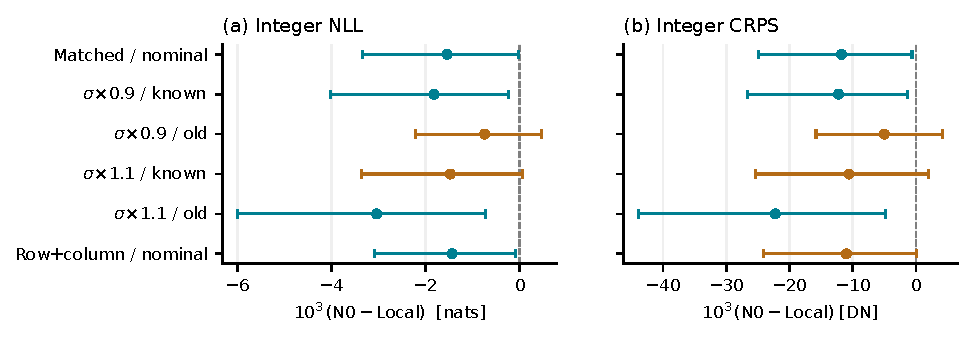
\includegraphics[width=\textwidth]{f09_paired_stress.pdf}
\caption{32 幅开发源图上的配对校准与相关噪声测试。每种设置使用两方法共享的 8,192 个中心零码候选。点为先按 CFA、再按源图汇总的均值差，误差条为 95\% 源图 bootstrap 区间，负值表示 N0 更低。图中已知设置向两种估计器及其解码器提供变化后的参数，原参数设置保留原校准。行、列偏移不提供给算法，橙色区间跨零。}
\label{fig:pairedstress}
\end{figure*}

\subsection{运行时间与资源表}
\begin{table}[tbp]
\centering
\caption{内存中处理的实现成本。不含解码、初始化和文件输出，数值后端与预热差别见正文。}
\label{tab:runtime}
\footnotesize\setlength{\tabcolsep}{4pt}
\begin{tabular}{@{}lrr@{}}
\toprule
指标 & N0/PG & Local PG $3\times3$\\
\midrule
128 打包像素中位时间 (s) & 0.2074 & 0.7329\\
24MP 三次中位时间 (s) & 27.3901 & 205.1503\\
24MP 时间范围 (s) & 25.1087--27.9992 & 194.3892--219.9394\\
CUDA 已分配 (MiB) & 750.69 & 94.84\\
CUDA 已保留 (MiB) & 1112.00 & 254.00\\
\bottomrule
\end{tabular}
\end{table}

表~\ref{tab:runtime} 报告了在单张 RTX 3090 Ti GPU（Python 3.10、PyTorch 2.6/CUDA 12.4、双 CPU 线程及显式 GPU 同步）上处理含 2,637,992 个零码的 24MP 输入的实测运行开销。小尺寸图像块测试采用 10 次预热与 30 次正式计时运行。在 24MP 全画幅测试中，N0 采用 10 次预热与 3 次正式运行，Local PG 则合并 1 次试运行与 2 次正式运行。实现后端方面，N0 采用 FP32 GPU 网络推理与 GPU LUT 线性插值，Local PG 采用 FP64 GPU 网格似然求值与 CPU LUT 插值，两者最终均在 CPU 上执行逆变换抽样。分块 Local PG 采用 128 像素核心块配 1 像素扩展边，在抽检的 32 个像素位置上，其与全图无分块执行的信号估计最大偏差低于 $3.05\times10^{-12}$ DN，LUT 离散概率质量函数完全一致，且分块最大似然估计距预设搜索网格上限至少留有 179.14 DN 的安全余量。

\subsection{成对校准与相关性分析}
我们在 32 幅开发源图生成的配对观测输入上系统对比了 N0 与同相位 $5\times5$ Local PG 的校准敏感性与相关噪声鲁棒性（实验采用 128 像素打包上下文、中心 64 像素评估区、每相位至多抽取 64 个零码，每种条件共含 8,192 个两方法共享的候选位置，评分先按 CFA 相位再按源图等权汇总，采用 10,000 次源图 bootstrap 重采样计算 95\% 置信区间）。当真实读出噪声标准差缩放为标称值的 $0.9$ 或 $1.1$ 倍时，我们分别测试向算法提供真实新参数（此时 N0 的常数校准通道需在训练点之外进行外推）与保留标称原参数两种设置，同时测试在观测中叠加标准差各为 5 DN 的未建模高斯行偏移与列偏移（由于真实生成律含空间相关性，该条件不报告超额 KL，整数评分通过解析 PG 尾部补齐）。

图~\ref{fig:pairedstress} 显示，在保留原参数的 $0.9\sigma$ 失配条件下，N0 减 Local PG 的成对 NLL 差值为 $-0.000746$ nats（95\% 区间 $[-0.002214,0.000462]$），已知参数 $1.1\sigma$ 条件下的置信区间同样跨零。而在未建模行、列条带偏移条件下，N0 减 Local PG 的成对 NLL 差值为 $-0.001439$ nats（95\% 区间 $[-0.003090,-0.000090]$），但相应的 CRPS 差值区间跨零。所有条件下的完整评分与稀有深尾敏感性测试均已归档。

\subsection{真实码事件范围}\label{sec:realcode}
实拍主评分覆盖两次曝光中全部 31,852 个共享候选像素。按嵌套负尾阈值 $V\leq-128$、$V\leq-256$ 和 $V\leq-305$ DN 统计，分别观测到 122、21 和 13 个极端负码事件，其中最极端的 13 个深尾事件对应原始相机文件码值 79--202 DN（经整数黑电平对齐后为 $-430$ 至 $-307$ DN）。两次独立曝光之间仅有 2 个像素坐标重复出现 $V\leq-128$ DN 的事件（其中 1 个坐标在两次曝光中均低于 $-305$ DN）。此外，两幅全画幅原始图像还分别独立包含 18 个和 25 个未经改动的原生零码（$R_{\mathrm{native}}=0$）。实拍噪声校准参数独立拟合自十幅全幅暗帧。尽管上述 13 个最深尾事件在两次曝光中分别使 N0 的绝对 NLL 显著增加了 0.03917 与 0.04525 nats，但它们对 N0 减 Local PG 成对 NLL 差值的净影响仅为 $+0.0000040$ 与 $-0.0000083$ nats。剔除全部 $V\leq-128$ DN 的极端事件后，两次曝光的成对 NLL 差值分别为 $-0.001375$ 与 $-0.000998$ nats（表~\ref{tab:real_robust}）。

在预先选定的 12 个固定实拍 ROI 中，N0 在其中 7 个 ROI 上取得更低的 NLL。对每个 ROI/CFA 单元执行对称 1\% 缩尾后，两次曝光的成对 NLL 差值分别为 $-0.001269$ 与 $-0.001082$ nats，与全样本未缩尾结果（$-0.001342$ 与 $-0.000964$ nats）高度吻合。共用 R/$G_1$ 噪声校准参数的诊断性 B 相位在两次曝光中的 N0 对 Local PG 平均 NLL 分别为 3.807768 对 3.810883 nats 以及 3.857925 对 3.859954 nats，全部逐 ROI 与逐 CFA 相位的详细评估记录均已归档。

\end{document}
